\documentclass[pdflatex,compress,mathserif]{beamer}

%\usetheme[dark,framenumber,totalframenumber]{ElektroITK}
\usetheme[darktitle,framenumber,totalframenumber]{ElektroITK}

\usepackage[utf8]{inputenc}
\usepackage[T1]{fontenc}
\usepackage{lmodern}
\usepackage[bahasai]{babel}
\usepackage{amsmath}
\usepackage{amsfonts}
\usepackage{amssymb}
\usepackage{graphicx}
\usepackage{multicol}
\setbeamertemplate{caption}[numbered]

\newcommand*{\Scale}[2][4]{\scalebox{#1}{$#2$}}%

\title{MATRIKULASI}
\subtitle{MATEMATIKA DASAR}

\author{Mifta Nur Farid}

\begin{document}

\maketitle

\section{Pengantar}

	\subsection{Pokok Bahasan}
		\begin{frame}{Pokok Bahasan}
			\begin{multicols}{2}
				\begin{enumerate}
					\item Pertidaksamaan Linier
					\begin{itemize}
						\item Interval
						\item Penyelesaian Pertidaksamaan
					\end{itemize}
					\item Fungsi dan Limit
					\begin{itemize}
						\item Fungsi
						\item Limit
					\end{itemize}
					\item Trigonometri
					\item Turunan
					\item Integral
					\begin{itemize}
						\item Integral Tak Tentu
						\item Integral dengan Substitusi
						\item Integral Tentu
					\end{itemize}
				\end{enumerate}
			\end{multicols}
		\end{frame}

\section{Pertidaksamaan Linier}

	\subsection{Interval}

		\begin{frame}
			\frametitle{Pertidaksamaan}
			\begin{itemize}
				\item Pertidaksamaan:
				\begin{equation}
					5x - 4 > 2x + 3
				\end{equation}
				\item Persamaan menggunakan simbol $ = $
				\item Pertidaksamaan menggunakan simbol
				\begin{center}
					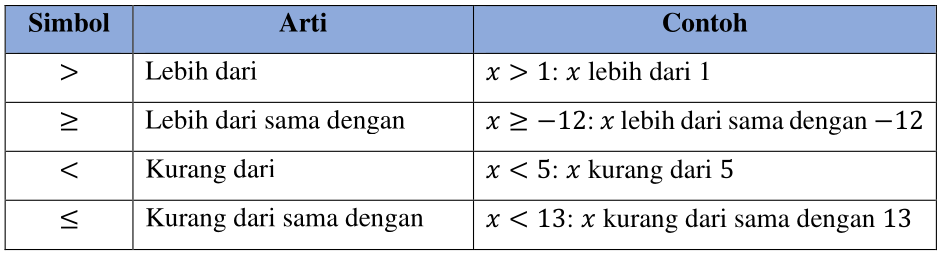
\includegraphics[width=\linewidth]{pict/01}
				\end{center}
			\end{itemize}
		\end{frame}
	
		\begin{frame}{Pertidaksamaan}
			\begin{itemize}
				\item Penyelesaian persamaan
				\begin{align*}
					5x - 4 &= 2x + 3\\
					5x - 2x &= 3 + 4\\
					3x &= 7\\
					x &= \frac{7}{3}
				\end{align*}
				\item Penyelesaian pertidaksamaan: rentang atau nilai variabel yang tidak diketahui yang memenuhi pertidaksamaan
			\end{itemize}
		\end{frame}
	
		\begin{frame}{Interval}
			\begin{itemize}
				\item Himpunan penyelesaian suatu pertidaksamaan dinyatakan dalam notasi himpunan atau bentuk selang atau \textit{interval}
				\item Jenis-jenis selang
				\begin{enumerate}
					\item Selang berhingga dan tertutup
					\item Selang berhingga dan terbuka
					\item Selang berhingga dan setengah terbuka atau setengah tertutup
					\item Selang tak hingga dan tertutup
					\item Selang tak hingga dan terbuka
					\item Selang tak hingga, terbuka, dan tertutup
				\end{enumerate}
			\end{itemize}
		\end{frame}
	
		\begin{frame}
			\frametitle{Selang berhingga dan tertutup}
			\begin{itemize}
				\item Notasi: $ [a,b] $
				\item Dinyatakan dalam notasi himpunan:
				\begin{equation}
					\{x:a \leq x \leq b\}
				\end{equation}
				\item Grafik selang:
				\begin{figure}
					\centering
					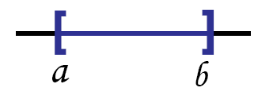
\includegraphics[width=0.5\linewidth]{pict/02}
					\caption{Grafik selang $[a,b]$}
					\label{fig:02}
				\end{figure}
			\end{itemize}
		\end{frame}
	
		\begin{frame}
			\frametitle{Selang berhingga dan terbuka}
			\begin{itemize}
				\item Notasi: $ (a,b) $
				\item Dinyatakan dalam notasi himpunan:
				\begin{equation}
					\{x:a < x < b\}
				\end{equation}
				\item Grafik selang:
				\begin{figure}
					\centering
					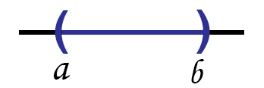
\includegraphics[width=0.5\linewidth]{pict/03}
					\caption{Grafik selang $(a,b)$}
					\label{fig:03}
				\end{figure}
			\end{itemize}
		\end{frame}
	
		\begin{frame}
			\frametitle{Selang berhingga dan setengah terbuka atau setengah tertutup}
			\begin{itemize}
				\item Notasi: $ (a,b] $ atau $ [a,b) $
				\item Notasi himpunan:
				\begin{align*}
					\text{Jika notasi } (a,b] & \text{, maka notasi himpunan }\{x:a < x \leq b\} \\
					\text{Jika notasi } [a,b) & \text{, maka notasi himpunan }\{x:a \leq x < b\} \\
				\end{align*}
				\item Grafik selang:
				\begin{multicols}{2}
					\begin{figure}
						\centering
						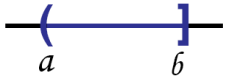
\includegraphics[width=0.5\linewidth]{pict/04}
						\caption{Grafik selang $(a,b]$}
						\label{fig:04}
					\end{figure}
					\columnbreak
					\begin{figure}
						\centering
						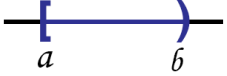
\includegraphics[width=0.5\linewidth]{pict/05}
						\caption{Grafik selang $[a,b)$}
						\label{fig:05}
					\end{figure}
				\end{multicols}
			\end{itemize}
		\end{frame}
		
		\begin{frame}
			\frametitle{Selang tak hingga dan tertutup}
			\begin{itemize}
				\item Notasi: $ [a,+\infty) $ atau $ (-\infty,b] $
				\item Notasi himpunan:
				\begin{align*}
					\text{Jika notasi } [a,+\infty) & \text{, maka notasi himpunan }\{x:x \geq a\} \\
					\text{Jika notasi } (-\infty,b] & \text{, maka notasi himpunan }\{x: x \leq b\} \\
				\end{align*}
				\item Grafik selang:
				\begin{multicols}{2}
					\begin{figure}
						\centering
						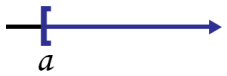
\includegraphics[width=0.5\linewidth]{pict/06}
						\caption{Grafik selang $[a,+\infty)$}
						\label{fig:06}
					\end{figure}
					\columnbreak
					\begin{figure}
						\centering
						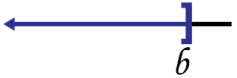
\includegraphics[width=0.5\linewidth]{pict/07}
						\caption{Grafik selang $(-\infty,b]$}
						\label{fig:07}
					\end{figure}
				\end{multicols}
			\end{itemize}
		\end{frame}
	
		\begin{frame}
			\frametitle{Selang tak hingga dan terbuka}
			\begin{itemize}
				\item Notasi: $ (a,+\infty) $ atau $ (-\infty,b) $
				\item Notasi himpunan:
				\begin{align*}
					\text{Jika notasi } (a,+\infty) & \text{, maka notasi himpunan }\{x:x > a\} \\
					\text{Jika notasi } (-\infty,b) & \text{, maka notasi himpunan }\{x: x < b\} \\
				\end{align*}
				\item Grafik selang:
				\begin{multicols}{2}
					\begin{figure}
						\centering
						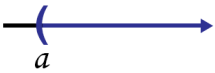
\includegraphics[width=0.5\linewidth]{pict/08}
						\caption{Grafik selang $(a,+\infty)$}
						\label{fig:08}
					\end{figure}
					\columnbreak
					\begin{figure}
						\centering
						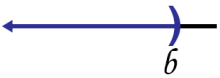
\includegraphics[width=0.5\linewidth]{pict/09}
						\caption{Grafik selang $(-\infty,b)$}
						\label{fig:09}
					\end{figure}
				\end{multicols}
			\end{itemize}
		\end{frame}
		
		\begin{frame}
			\frametitle{Selang tak hingga}
			\begin{itemize}
				\item Notasi: $ (-\infty,+\infty) $
				\item Notasi himpunan:
				\begin{equation*}
					\{ x : x \in \mathcal{R} \}
				\end{equation*}
				\item Grafik selang:
				\begin{figure}
					\centering
					
\includegraphics[width=0.5\linewidth]{pict/10}
					\caption{Grafik selang $(-\infty,+\infty)$}
					\label{fig:10}
				\end{figure}
			\end{itemize}
		\end{frame}
	
	\subsection{Penyelesaian Pertidaksamaan}
	
		\begin{frame}
			\frametitle{Penyelesaian pertidaksamaan}
			Hal-hal yang perlu diperhatikan dalam menyelesaikan suatu pertidaksamaan
			\begin{enumerate}
				\item Prosedur menyelesaikan pertidaksamaan adalah mengubah pertidaksamaan satu langkah demi satu langkah hingga diperoleh himpunan penyelesaiannya jelas.
				\item Dapat dilakukan operasi-operasi tertentu (tambah, kurang, kali, bagi, akar, pangkat) pada kedua ruas pada suatu pertidaksamaan. Perlakuan pada kedua ruas harus sama, contohnya:
				\begin{enumerate}
					\item Kedua ruas ditambah atau dikurangi dengan suatu bilangan;
					\item Kedua ruas dikali atau dibagi dengan suatu bilangan positif;
					\item Jika kedua ruas dikali atau dibagi dengan bilangan negatif, tanda pertidaksamaan harus berbalik arah.
				\end{enumerate}
			\end{enumerate}
		\end{frame}
	
	\subsection{Contoh Soal}
	
		\begin{frame}
			\frametitle{Contoh 1}
			Selesaikan pertidaksamaan
			\begin{equation*}
				-5x - 10 < 15
			\end{equation*}
			dan tunjukkan garis bilangan himpunan penyelesaiannya.
		\end{frame}
	
		\begin{frame}
			\frametitle{Jawaban Contoh 1}
			\begin{align*}
				-5x - 10 & < 15 &\\
				-5x - 10 + 10 & < 15 + 10 & \text{(kedua ruas ditambah 10)} \\
				-5x & < 25 & \\
				\frac{-5x}{-5} & > \frac{25}{-5} & \text{(kedua ruas dikali dengan } -\frac{1}{5} \text{)}\\
				x & > -5
			\end{align*}
		\end{frame}
		
		\begin{frame}{Jawaban Contoh 1}
			\begin{itemize}
				\item Himpunan penyelesaiannya adalah $ \{ x : x > -5 \} $, atau \item Dalam bentuk selang $ (-5,+\infty) $.
				\item Berikut $ (-5,+\infty) $ diinterpretasikan dalam bentuk garis bilangan.
				\begin{figure}
					\centering
					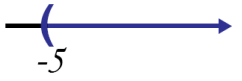
\includegraphics[width=0.3\linewidth]{pict/11}
					\caption{Grafik selang $(-5,+\infty)$}
					\label{fig:11}
				\end{figure}
			\end{itemize}
		\end{frame}
		
		\begin{frame}
			\frametitle{Contoh 2}
			Selesaikan pertidaksamaan
			\begin{equation*}
				-5 \leq 2x + 6 < 4
			\end{equation*}
			dan tunjukkan garis bilangan himpunan penyelesaiannya.
		\end{frame}
	
		\begin{frame}
			\frametitle{Jawaban Contoh 2}
			\begin{tabular}{rcccll}
				$ -5 $ & $\leq$ & $ 2x + 6 $ & < & $ 4 $ &  \\
				$ -5-6 $ & $\leq$ & $ 2x + 6 - 6 $ & < & $ 4 - 6 $ & (dikurangin 6) \\
				$ -11 $ & $\leq$ & $ 2x $ & < & $ -2 $ & \\
				$-11/2$ & $\leq$ & $2x/2$ & < & $-2/2$ & (dibagi 2 atau dikali $\frac{1}{2}$)\\
				$ -11/2 $ & $\leq$ & $ x $ & < & $ -1 $ &  \\
			\end{tabular}
		\end{frame}
		
		\begin{frame}{Jawaban Contoh 2}
			Himpunan penyelesaiannya adalah
			\begin{equation*}
				\left\{ x:-\frac{11}{2} \leq x < -1 \right\}
			\end{equation*}
			atau ditulis dalam bentuk selang $ \left[ -\frac{11}{2}, -1 \right) $ atau dengan garis bilangan
			\begin{figure}
				\centering
				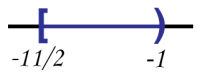
\includegraphics[width=0.3\linewidth]{pict/12}
				\caption{Grafik selang $ \left[ -\frac{11}{2}, -1 \right) $ }
				\label{fig:12}
			\end{figure}
		\end{frame}
		
		\begin{frame}
			\frametitle{Contoh 3}
			Selesaikan pertidaksamaan 
			\begin{equation*}
				x^2 - x < 6
			\end{equation*}
		\end{frame}
	
		\begin{frame}
			\frametitle{Jawaban Contoh 3}
			\begin{align*}
				x^2 - x &< 6 &\\
				x^2 - x - 6 & < 6 - 6 & \text{(dikurangi 6)}\\
				(x+2)(x-3)& <  0 &\text{(difaktorkan)}\\
			\end{align*}
			\begin{itemize}
				\item Dapat dilihat bahwa $ x = -2 $ dan $ x = 3 $ membagi garis bilangan kedalam tiga selang terbuka yaitu $ (-\infty, -2) $, $ (-2,3) $, dan $ (3, +\infty) $.
				\item Selanjutnya kita harus mengecek setiap tanda diselang dengan cara diambil satu titik yang berada di tiga selang tersebut.
			\end{itemize}
		\end{frame}
	
		\begin{frame}{Jawaban Contoh 3}
			\begin{itemize}
				\item $ x = -3 $ mewakili titik yang berada pada selang $ (-\infty, -2) $
				\item $ x = 0 $ mewakili titik yang berada pada selang $ (-2, 3) $
				\item $ x = 5 $ mewakili titik yang berada pada selang $ (3, +\infty) $
				\begin{figure}
					\centering
					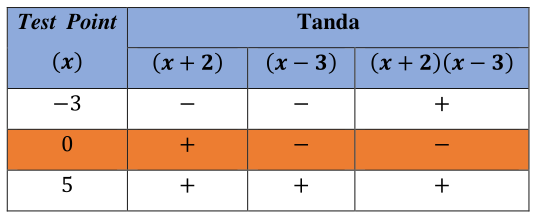
\includegraphics[width=0.7\linewidth]{pict/13}
				\end{figure}
				\item Daerah yang memenuhi $ (x+2)(x-3)<0 $ adalah selang $ (-2,3) $
			\end{itemize}
			
		\end{frame}
	
		\begin{frame}{Jawaban Contoh 3}
			Himpunan penyelesaiannya adalah
			$$ \{x: -2 < x < 3\} $$
			atau dalam bentuk selang $ (-2,3) $ atau dengan garis bilangan
			\begin{figure}
				\centering
				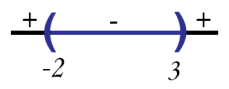
\includegraphics[width=0.3\linewidth]{pict/14}
				\caption{Grafik selang $ (-2,3) $ dan tanda di masing-masing daerahnya}
				\label{fig:14}
			\end{figure}
		\end{frame}
	
		\begin{frame}
			\frametitle{Contoh 4}
			Selesaikan pertidaksamaan
			\begin{equation*}
				3x^2 - x - 2 \geq 0
			\end{equation*}
		\end{frame}
	
		\begin{frame}
			\frametitle{Jawaban Contoh 4}
			\begin{align*}
				3x^2 - x - 2 &\geq 0 &\\
				(x-1)(3x+2) &\geq 0 & \text{(difaktorkan)}
			\end{align*}
			\begin{itemize}
				\item Dapat dilihat bahwa $ x = -\frac{2}{3}$ dan $ x = 1 $ membagi garis bilangan ke dalam tiga selang tertutup yaitu $ (-\infty, -\frac{2}{3}] $, $ [-\frac{2}{3} , 1] $, dan $ [1, +\infty) $.
			\end{itemize}
		\end{frame}
	
		\begin{frame}{Jawaban Contoh 4}
			\begin{itemize}
				\item Uji tanda
				\begin{figure}
					\centering
					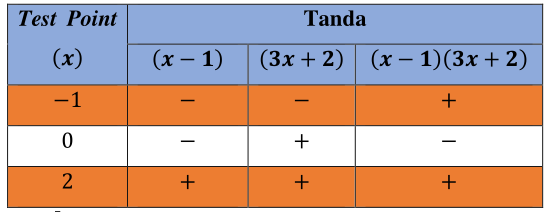
\includegraphics[width=0.7\linewidth]{pict/15}
				\end{figure}
			\end{itemize}
		\end{frame}
	
		\begin{frame}{Jawaban Contoh 4}
			Himpunan penyelesaiannya adalah
			$$ \{x: x \leq -\frac{2}{3} \cup x \geq 1\} $$
			atau dalam bentuk selang $ \left(-\infty,-\frac{2}{3} \right] \cup \left[ 1,+\infty \right) $ atau dengan garis bilangan
			\begin{figure}
				\centering
				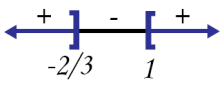
\includegraphics[width=0.3\linewidth]{pict/16}
				\caption{Grafik selang $ \left(-\infty,-\frac{2}{3} \right] \cup \left[ 1,+\infty \right) $ dan tanda di masing-masing daerahnya}
				\label{fig:16}
			\end{figure}
		\end{frame}
	
		\begin{frame}
			\frametitle{Contoh 5}
			Selesaikan pertidaksamaan
			\begin{equation*}
				\frac{x - 1}{x + 2} \geq 0
			\end{equation*}
		\end{frame}
		
		\begin{frame}
			\frametitle{Jawaban Contoh 5}
			\begin{itemize}
				\item Perhatikan masing-masing persamaan yang menjadi pembilang dan penyebut saat sama dengan nol.
				\begin{itemize}
					\item Nilai $ x - 1 = 0 $ jika $ x = 1 $
					\item Nilai $ x + 2 = 0 $ jika $ x = -2 $
				\end{itemize}
				\item $ x = 1 $ dan $ x = -2 $ menghasilkan 3 selang yaitu $ (-\infty,-2) $, $ (-2,1] $, dan $ [1,+\infty) $
				\begin{itemize}
					\item Selang $ (-\infty,-2) $ tidak tertutup di $ x = -2 $ karena apabila disubstitusikan $ x = -2 $ ke persamaan $\frac{x-1}{x+2}$ akan membuat penyebutnya bernilai nol.
				\end{itemize}
				\item Selanjutnya dilakukan uji tanda
			\end{itemize}
		\end{frame}
	
		\begin{frame}{Jawaban Contoh 5}
			\begin{itemize}
				\item Uji tanda
				\begin{figure}
					\centering
					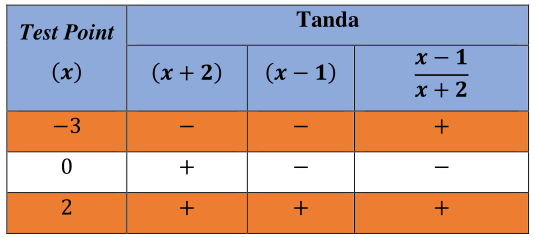
\includegraphics[width=0.7\linewidth]{pict/17}
				\end{figure}
			\end{itemize}
		\end{frame}
		
		\begin{frame}{Jawaban Contoh 5}
			Himpunan penyelesaiannya adalah
			$$ \{x: x \leq -2 \cup x \geq 1\} $$
			atau dalam bentuk selang $ \left(-\infty,-2 \right) \cup \left[ 1,+\infty \right) $ atau dengan garis bilangan
			\begin{figure}
				\centering
				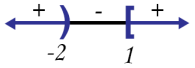
\includegraphics[width=0.3\linewidth]{pict/18}
				\caption{Grafik selang $ \left(-\infty,-2 \right) \cup \left[ 1,+\infty \right) $ dan tanda di masing-masing daerahnya}
				\label{fig:18}
			\end{figure}
		\end{frame}
	
	\subsection{Latihan Soal}
	
	\begin{frame}
		\frametitle{Latihan Soal}
		Selesaikan pertidaksamaan dibawah ini dan sketsakan himpunan penyelesaiannya pada garis koordinat:
		\begin{enumerate}
			\item $ 3x - 5 > -7x -4 $
			\item $ 2(x+3) < x + 1 $
			\item $ 1 \leq 2 - 3x < 8 $
			\item $ 2x^2 + 3x - 2 \leq 0 $
			\item $ \frac{2}{x - 5} \geq \frac{1}{x + 1}$
		\end{enumerate}
	\end{frame}
	
\section{Fungsi Dan Limit}

	\subsection{Fungsi}
	
		\begin{frame}
			\frametitle{Fungsi}
			\begin{itemize}
				\item Sebuah fungsi $ f $ adalah suatu aturan korespondensi yang menghubungkan setiap objek $ x $ dalam satu himpunan yang disebut daerah asal/domain, dengan sebuah nilai tunggal $ f(x) $ dari suatu himpunan kedua (kodomain).
				\item Himpunan nilai yang diperoleh dari $ f(x) $ disebut daerah hasil/range.
				\item Umumnya, fungsi dinotasikan sebagai $ y = f(x) $ dengan $ x $ adalah peubah (variabel) bebas dari $ f $ yang merupakan domain, sedangkan $ y $ merupakan peubah (variable tak bebas) dari $ y $.
				\begin{itemize}
					\item Berarti nilai $ y $ yang dihasilkan bergantung pada nilai $ x $ yang diberikan.
				\end{itemize}
				\item Nilai-nilai $ x $ merupakan anggota dari domain fungsi $ f $ dan $ y $ merupakan anggota dari range fungsi $ f $.
			\end{itemize}
		\end{frame}
	
		\begin{frame}{Fungsi}
			\begin{itemize}
				\item Jika didefinisikan fungsi $ y = f(x) $, maka domain (daerah asal) dari $ f $ merupakan himpunan nilai – nilai dari himpunan bebas (variabel) $ x $ yang dinotasikan sebagai $ D_f $.
				\item Sedangkan range merupakan semua nilai $ f(x) $ untuk setiap $ x $ pada domain $ f $. Range dari fungsi $ f $ dinotasikan sebagai $ R_f $ .
			\end{itemize}
		\end{frame}
	
		\begin{frame}{Fungsi}
			\begin{itemize}
				\item Diberikan dua buah fungsi $ f $ dan $ g $, maka rumus-rumus untuk jumlah $ f+g $, selisih $ f-g $, hasil kali $ f \cdot g $, dan hasil bagi $ \frac{f}{g} $ didefinisikan sebagai
				\begin{align*}
					(f+g)(x) &= f(x) + g(x) \\
					(f-g)(x) &= f(x) - g(x) \\
					(f \cdot g)(x) &= f(x) \cdot g(x) \\
					\left( \frac{f}{g} \right)(x) &= \frac{f(x)}{g(x)},~g(x) \neq 0
				\end{align*}
				\item Komposisi fungsi $ f $ dan $ g $ dinyatakan sebagai berikut
				\begin{equation*}
					(f \circ g)(x) = f(g(x))
				\end{equation*}
				atau dinotasikan $ f \circ g $
			\end{itemize}
		\end{frame}
		
		\begin{frame}
			\frametitle{Contoh 1}
			Diberikan suatu fungsi $ f(x) = x^2 - 2x $, tentukan dan sederhanakan nilai dari
			\begin{enumerate}
				\item $ f(x) $
				\item $ f(4+h) $
				\item $\frac{f(4+h) - f(4)}{h}$
			\end{enumerate}
		\end{frame}
	
		\begin{frame}
			\frametitle{Jawaban Contoh 1}
			\begin{enumerate}
				\item $ f(x) $
				\item $ f(4+h) $
				\item $\frac{f(4+h) - f(4)}{h}$
			\end{enumerate}
		\end{frame}
	
	\subsection{Limit}

\section{Trigonometri}

\section{Turunan}

\section{Integral}

	\subsection{Integral Tak Tentu}

	\subsection{Integral dengan Substitusi}
	
	\subsection{Integral Tentu}

\end{document}
